% Changing book to article will make the footers match on each page,
% rather than alternate every other.
\documentclass[10pt,twoside,twocolumn,openany]{book}
\usepackage[bg-letter]{dnd} % Options: bg-a4, bg-letter, bg-full, bg-print, bg-none.
\usepackage[english]{babel}
\usepackage[utf8]{inputenc}

% Start document
\begin{document}
\fontfamily{ppl}\selectfont % Set text font

% Your content goes here

\onecolumn
\chapter{Hotel Archimedes}
\begin{figure}[h!]
    \centering
    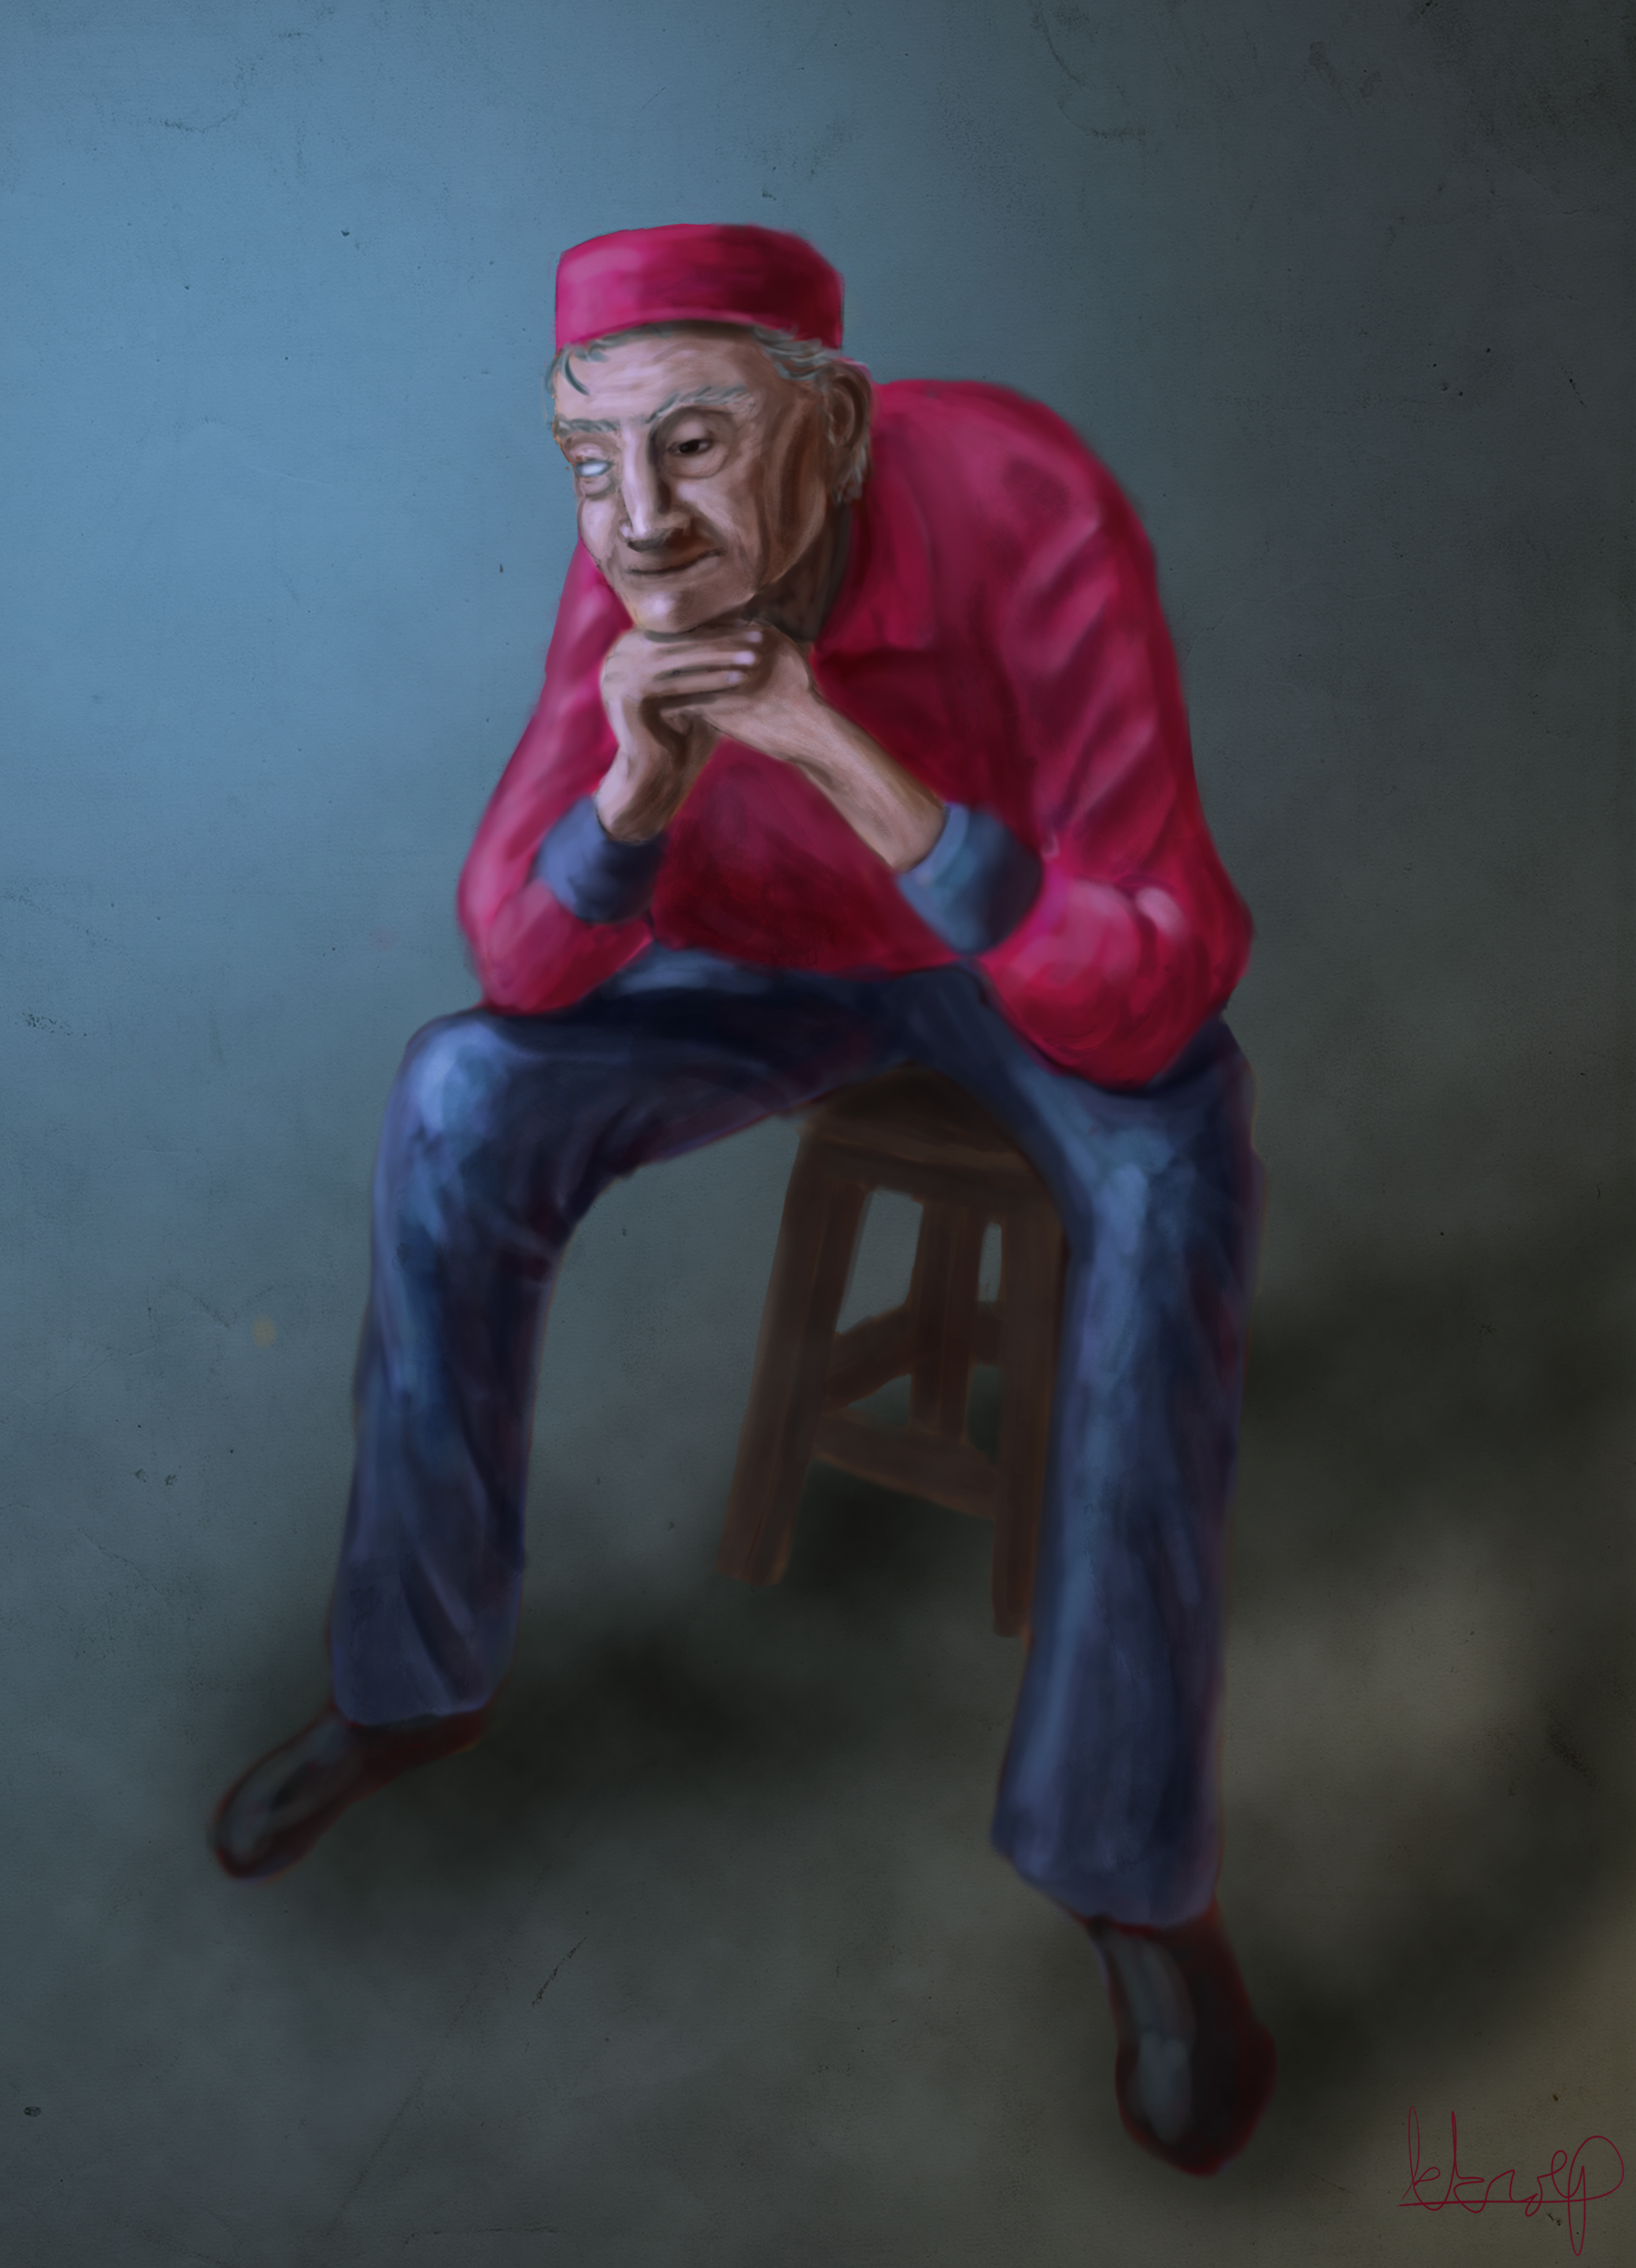
\includegraphics[width = 0.7\textwidth]{img/hunchback.png}
    \caption{<+caption text+>}
    \label{fig:<+label+>}
\end{figure}



\tableofcontents

\clearpage
\twocolumn

\section{Introduction}
\lipsum[1] % filler text

\section{Notes for DM}
\lipsum[1]

\section{Milstones}
\lipsum[1]






\section{Some example structures}
\subsection{Fun with boxes}
\subsubsection{Even more fun!}


\subtitlesection{Weapon, +1, +2, or +3}
{Weapon (any), uncommon (+1), rare (+2), or very rare (+3)}

\newpage % Acts as columbreak because of twocolumn option; for pagebreak use \clearpage

\header{Nice table}
\begin{dndtable}
   	\textbf{Table head}  & \textbf{Table head} \\
   	Some value  & Some value \\
   	Some value  & Some value \\
   	Some value  & Some value
\end{dndtable}



% End document
\end{document}
